%%%%%%%%%%%%%%%%%%%%%%%%%%%%%%%%%%%%%%%%%%%%%%%%%%%%%%%%%
% Niniejszy plik przedstawia przykładowy skład 
% pracy dyplomowej na Wydziale Matematyki PWr. 
% 
% Autorzy: 
% Damian Fafuła
% Michał Kijaczko
% Jakub Michalczak
% Maciej Miśta
% Dagmara Nowak
% Tomasz Skalski
% Wojciech Słomian
%
%% Data utworzenia: 8.05.2018
% Numer wersji: 1
%
% Poniższą formatkę można rozpowszechniać i edytować 
% pod warunkiem zachowania numeru wersji, 
% informacji o autorach i dodaniu informacji 
% o wprowadzonych zmianach.
%
%%%%%%%%%%%%%%%%%%%%%%%%%%%%%%%%%%%%%%%%%%%%%%%%%%%%%%%%%
% Domyślną opcją jest: praca magisterska, język polski.
% W przypadku pracy pisanej w języku angielskim dodajemy 
% opcję [english].
% Dla pracy licencjackiej dodajemy opcję [licencjacka].
% Dla pracy inżynierskiej dodajemy opcję [inzynierska].
% Dopuszczalne są podwójne opcje, np. [licencjacka, english].
% Opcje dodajemy w kwadratowym nawiasie przy \documentclass.
%
%
%%%%%%%%%%%%%%%%%%%%%%%%%%%%%%%%%%%%%%%%%%%%%%%%%%%%%%%%%
\documentclass[magisterska, english]{pwr_wmat_praca_dyplomowa}
\frenchspacing 
%%%%%%%%%%%%%%%%%%%%%%%%%%%%%%%%%%%%%%%%%%%%%%%%%%%%%%%%%
%              DANE DO PRACY
%
% W przypadku pracy dyplomowej w języku angielskim nie jest konieczne 
% wypełnianie pól: \tytul{}, \kierunek{}, \specjalnosc{}, 
%                  \streszczenie{}, \slowakluczowe{}.
%%%%%%%%%%%%%%%%%%%%%%%%%%%%%%%%%%%%%%%%%%%%%%%%%%%%%%%%%
%
% Imię i nazwisko autora
\autor{Aleksander Jakóbczyk}
%
% Tytuł pracy dyplomowej 
\tytul{Sequential methods for A/B testing} 
\tytulang{Sequential methods for A/B testing}
%
% Tytuł / stopień / imię i nazwisko opiekuna
\opiekun{dr inż. Andrzej Giniewicz}
%
% Kierunek studiów wybieramy spośród następujących:
% 1) Matematyka
% 2) Matematyka i Statystyka
% 3) Matematyka stosowana
\kierunekstudiow{Matematyka stosowana}
%
% Kierunek studiów po angielsku wybieramy spośród następujących:
% 1) Mathematics
% 2) Mathematics and Statistics
% 3) Applied Mathematics
\kierunekstudiowang{Applied Mathematics}
%
% Specjalność wybieramy spośród następujących: 
% KIERUNEK: Matematyka
% 1) Matematyka teoretyczna,
% 2) Statystyka matematyczna,
% 3) Matematyka finansowa i ubezpieczeniowa,
%
% KIERUNEK: Matematyka i Statystyka
% 4) Matematyka,
% 5) Statystyka i analiza danych, 
%
% 6) -- (w przypadku braku specjalizacji).
\specjalnosc{--} 
%
% Specjalność w języku angielskim wybieramy spośród następujących:
% KIERUNEK: Matematyka
% 1) Theoretical Mathematics,
% 2) Mathematical Statistics,
% 3) Financial and Actuarial Mathematics,
%
% KIERUNEK: Matematyka i Statystyka
% 4) Mathematics,
% 5) Statistics and Data Analysis,
%
% KIERUNEK: Applied Mathematics
% 6) Financial and Actuarial Mathematics, 
% 7) Mathematics for Industry and Commerce,
% 8) Computational Mathematics,
% 9) Modelling, Simulation and Optimization.
%
% 10) -- (w przypadku braku specjalizacji).
\specjalnoscang{Data Engineering} 
%
% Krótkie streszczenia po polsku i angielsku
% - nie dłuższe niż 530 znaków.

\streszczenie{TODO}
\streszczenieang{TODO}
%TODO aold \streszczenie{Celem pracy jest wyznaczenie nieoczekiwanych strategii w grach częściowo obserwowalnych za pomocą metod stochastycznej optymalizacji.
%	%! wstemp do poprawy
%	W pracy zostały zaproponowane nowe algorytmy, pozwalające na szybsze wyznaczenie strategii optymalnej. Zaproponowano również kolejny algorytm generacyjny. Przeprowadzona została analiza porównawcza kilku wybranych metod optymalizacji.}
%\streszczenieang{The aim of this work is to determine unexpected strategies in partially observable games using stochastic optimization methods. New algorithms have been proposed to allow for faster determination of the optimal strategy. Another generative algorithm has been proposed. A comparative analysis of several optimization methods was conducted.}
%
% Podajemy najważniejsze słowa kluczowe po polsku i angielsku
% - w obu przypadkach, nie więcej niż 150 znaków.
\slowakluczowe{}  
\slowakluczoweang{}
%TODO \slowakluczowe{gry częściowo obserwowalne,
%	strategia optymalna,
%	stochastyczna optymalizacja,
%	Hoeffding race,
%	empirical Bernstein race,
%	algorytmy genetyczne.}  
%\slowakluczoweang{partially observable game,
%	optimal strategy,
%	stochastic optimization,
%	Hoeffding race,
%	empirical Bernstein race,
%	genetic algorithm}
%
%
%%%%%%%%%%%%%%%%%%%%%%%%%%%%%%%%%%%%%%%%%%%%%%%%%%%%%%%%%
% Definicje, lematy, twierdzenia, przykłady i wnioski
% Komendy wywołujące twierdzenia, definicje, itd., 
% czyli 'theorem', 'definition', 'corollary', itd., 
% można zmienić wedle uznania.
\theoremstyle{plain}
\newtheorem{theorem}{Theorem}
\numberwithin{theorem}{chapter}
\newtheorem{lemma}[theorem]{Lemma} 
\newtheorem{corollary}[theorem]{Corollary}
\newtheorem{fact}[theorem]{Fact}
\theoremstyle{definition}
\numberwithin{theorem}{chapter}
\newtheorem{definition}[theorem]{Definition} 
\newtheorem{example}[theorem]{Example}
\newtheorem{note}[theorem]{Note}
%%%%%%%%%%%%%%%%%%%%%%%%%%%%%%%%%%%%%%%%%%%%%%%%%%%%%%%%%

\usepackage{amsmath}
\usepackage{amsthm}
\usepackage{amsfonts}
\usepackage{amssymb}
\usepackage{graphicx}
\usepackage{caption}
\usepackage{xcolor}
\usepackage{algpseudocode,algorithm,algorithmicx}
\usepackage{enumitem}
%\usepackage[plmath]{polski}
\newcommand{\pauza}{---}
\newcommand{\ppauza}{--}

\usepackage{booktabs}
\usepackage{icomma}
\usepackage{indentfirst}

\usepackage{subcaption}
\usepackage{hyperref}




\addto\captionsenglish{\renewcommand{\figurename}{Figure}}

\DeclareMathOperator*{\argmax}{arg\,max}
\DeclareMathOperator*{\argmin}{arg\,min}


\DeclareRobustCommand{\bbone}{\text{\usefont{U}{bbold}{m}{n}1}}
\DeclareMathOperator{\EX}{\mathbb{E}}% expected value
\DeclareMathOperator{\Var}{\mathrm{Var}}% 
\DeclareCaptionLabelFormat{custom}
{%
	Algorithm \thealgorithm:
}
\newcommand{\probP}{\mathbb{P}}
\newcommand{\nmax}{n_{\text{max}}}
\newcommand{\nmin}{n_{\text{min}}}
\newcommand{\tmin}{t_{\text{min}}}
\newcommand{\tmax}{t_{\text{max}}}

\newcommand{\newbrackets}[1]{\emph{(}{#1}\emph{)}}


\newenvironment{polishalgorithm}[1][]
{\begin{algorithm}[#1]
		\floatname{algorithm}{Algorithm}%
		
		\newcommand{\obtain}{Realizacja }%
		\newcommand{\precision}{precyzja }%
		\newcommand{\probability}{prawdopodobienstwo }%
		\newcommand{\randomopponent}{losowy przeciwnik }%
		\newcommand{\find}{Znajdz }%
		\newcommand{\suchas}{\!\!, takie że }%
		\newcommand{\algand}{i }%
		\newcommand{\algor}{lub }%
		\newcommand{\win}{lepszy }%
		\newcommand{\tolenghtof}{do długości }%
		\newcommand{\playgamebetween}{rozegraj grę pomiędzy }%
		\newcommand{\betterthen}{lepszy niż }%
		\newcommand{\allpointsin}{wszystkie punkty z }%
		\newcommand{\better}{lepszy}%
		
		
		%\newcommand{\individualofP}{$rand^\text{th}$ individual of P}%
		\newcommand{\individualofP}{$P_k$}%
		
		%\newcommand{\drawrandom}{Draw at random an integer $rand$ between 1 \algand the size of $P$}%
		\newcommand{\drawrandom}{k $\gets$ liczba naturalna z przedziału od $1$ do długości $P$}%
		
		%\newcommand{\randomindividualof}{random individual of }%
		\newcommand{\randomindividualof}{losową strategia z }%
		
		%\newcommand{\approximationx}{\approximationx }%
		\newcommand{\approximationx}{przybliżoną strategię optymalną $x$}%
		
		%\newcommand{\bernsteinnotstop}{the limited Bernstein race of precision ${\ep}silon$ not stop}
		\newcommand{\bernsteinnotstop}{ILEBR* 2 trawa}
		
		%\newcommand{\termination}{(termination criterion is not met)}
		\newcommand{\termination}{(kryterium zakończenia nie jest spełnione)}
		
		%\newcommand{\obtainfirstgames}[1]{Obtain first {##1} games}%
		\newcommand{\obtainfirstgames}[1]{Realizacja pierwszych {##1} gier}%
		
		
		\renewcommand{\algorithmicensure}{\textbf{Wprowadź:}}%
		\renewcommand{\algorithmicwhile}{\textbf{dopóki}}%
		\renewcommand{\algorithmicdo}{\textbf{wykonaj}}%
		\renewcommand{\algorithmicreturn}{\textbf{zwróć}}%
		\renewcommand{\algorithmicif}{\textbf{jeżeli}}%
		\renewcommand{\algorithmicthen}{\textbf{to}}%
		\renewcommand{\algorithmicelse}{\textbf{w przeciwnym\ razie}}%
		\renewcommand{\algorithmicfor}{\textbf{dla każdego}}%
		\algrenewtext{ElsIf}[1]{\textbf{jeśli jednak} {##1} \algorithmicthen }
		\algrenewtext{ForAll}[1]{\textbf{dla każdego} {##1} \algorithmicdo}
		\renewcommand{\algorithmicend}{\textbf{koniec}}%

	}
	{\end{algorithm}}
%%%%%%%%%%%%%%%%%%%%%%%%%%%%%%%%%%%%%%%%%%%%%%%%%%%%%%%%%
%%%%%%%%%%%%%%%%%%%%%%%%%%%%%%%%%%%%%%%%%%%%%%%%%%%%%%%%%
\begin{document}
\frontmatter
\maketitle
\mainmatter
\tableofcontents
%\listoffigures
%\listoftables
{\backmatter \chapter{Introduction}} 

\chapter{Concepts, Theorems, and Literature in A/B Testing}
%TODO dodaj opistego cahpteru


\section{Classical A/B Testing}

Classical A/B testing, also known as split testing, is a fundamental technique in experimental design, widely used to compare two versions of a product, feature, or strategy. Typically, these are labeled as variant A (control) and variant B (treatment). The primary objective is to determine which variant performs better according to a specific metric, such as conversion rate, click-through rate, or user engagement. This approach is integral to data-driven decision-making processes, particularly in digital marketing, web development, and user experience optimization \cite{Kohavi2007}.

\subsection{Theoretical Foundations}

The theoretical foundations of classical A/B testing are deeply rooted in the principles of statistical hypothesis testing. This methodology provides a rigorous framework for determining whether observed differences between two groups are statistically significant or merely due to random variation \cite{Fisher1925}.

Let \( X_A \) and \( X_B \) represent the observed outcomes for the control and treatment groups, respectively. These outcomes are assumed to be independent and identically distributed (i.i.d.) random variables:
\[
X_A = \{X_{A1}, X_{A2}, \dots, X_{A n_A}\}, \quad X_B = \{X_{B1}, X_{B2}, \dots, X_{B n_B}\}.
\]

The objective of the A/B test is to test the null hypothesis \( H_0 \), which posits that the population means of the two groups are equal:

\[
H_0: \mu_A = \mu_B,
\]
against the alternative hypothesis \( H_1 \):

\[
H_1: \mu_A \neq \mu_B.
\]

This hypothesis test is typically conducted using a two-sample t-test, which compares the sample means \( \bar{X}_A \) and \( \bar{X}_B \). The test statistic \( T \) is defined as:

\[
T = \frac{\bar{X}_A - \bar{X}_B}{\sqrt{s_p^2\left(\frac{1}{n_A} + \frac{1}{n_B}\right)}},
\]
where \( s_p^2 \) is the pooled sample variance, calculated as:

\[
s_p^2 = \frac{(n_A - 1)s_A^2 + (n_B - 1)s_B^2}{n_A + n_B - 2},
\]
with \( s_A^2 \) and \( s_B^2 \) being the sample variances, and \( n_A \), \( n_B \) representing the sample sizes for the control and treatment groups, respectively. Under the null hypothesis \( H_0 \), the test statistic \( T \) follows a t-distribution with \( n_A + n_B - 2 \) degrees of freedom \cite{Rice2006}.

The decision rule for the t-test is based on a significance level \( \alpha \), typically set at 0.05. If the computed value of \( |T| \) exceeds the critical value \( t_{\alpha/2, \nu} \) from the t-distribution, where \( \nu = n_A + n_B - 2 \), the null hypothesis \( H_0 \) is rejected in favor of the alternative hypothesis \( H_1 \). This indicates that the difference between the two group means is statistically significant \cite{Student1908}.


\subsection{Practical Considerations}

While the theoretical framework of classical A/B testing is robust, its practical implementation requires careful consideration of several factors. A critical aspect is ensuring that the randomization process is genuinely random. Any bias in the assignment of subjects to the control and treatment groups can lead to confounding variables and biased estimates of treatment effects \cite{Kohavi2013}. Ensuring true randomization is essential for maintaining the independence of observations, which is a key assumption of the t-test.

Another crucial consideration is determining the appropriate sample size. The power of a statistical test—the probability of correctly rejecting a false null hypothesis—depends on the sample size, the effect size $\Delta = |\mu_A - \mu_B|$, and the variance $\sigma^2$. The required sample size for a two-sample t-test can be calculated as:

\[
n = \frac{2\sigma^2(Z_{\alpha/2} + Z_\beta)^2}{\Delta^2},
\]
where $Z_{\alpha/2}$ and $Z_\beta$ are the critical values from the standard normal distribution corresponding to the significance level $\alpha$ and the desired power $(1-\beta)$, respectively \cite{Cohen1988}. A well-powered study increases the likelihood of detecting a true effect, while an underpowered study may fail to do so, leading to a Type II error (false negative). Conversely, an overpowered study may detect trivial differences that are not practically significant, leading to a Type I error (false positive) \cite{Sullivan2012}.

\subsection{Power Analysis}

The power of a statistical test is a crucial consideration in the design of an A/B test. Power is defined as the probability of correctly rejecting the null hypothesis when it is false, and it depends on the effect size, sample size, significance level, and population variance \cite{Cohen1988}. To visualize how these factors influence the power of the test, we can generate a power curve.

Figure~\ref{fig:power_curve} illustrates the relationship between the effect size $\Delta$ and the power of the test for various sample sizes. As shown in the figure, larger sample sizes and larger effect sizes both lead to increased power, meaning the test is more likely to detect a true effect.

\begin{figure}[H]
	\centering
	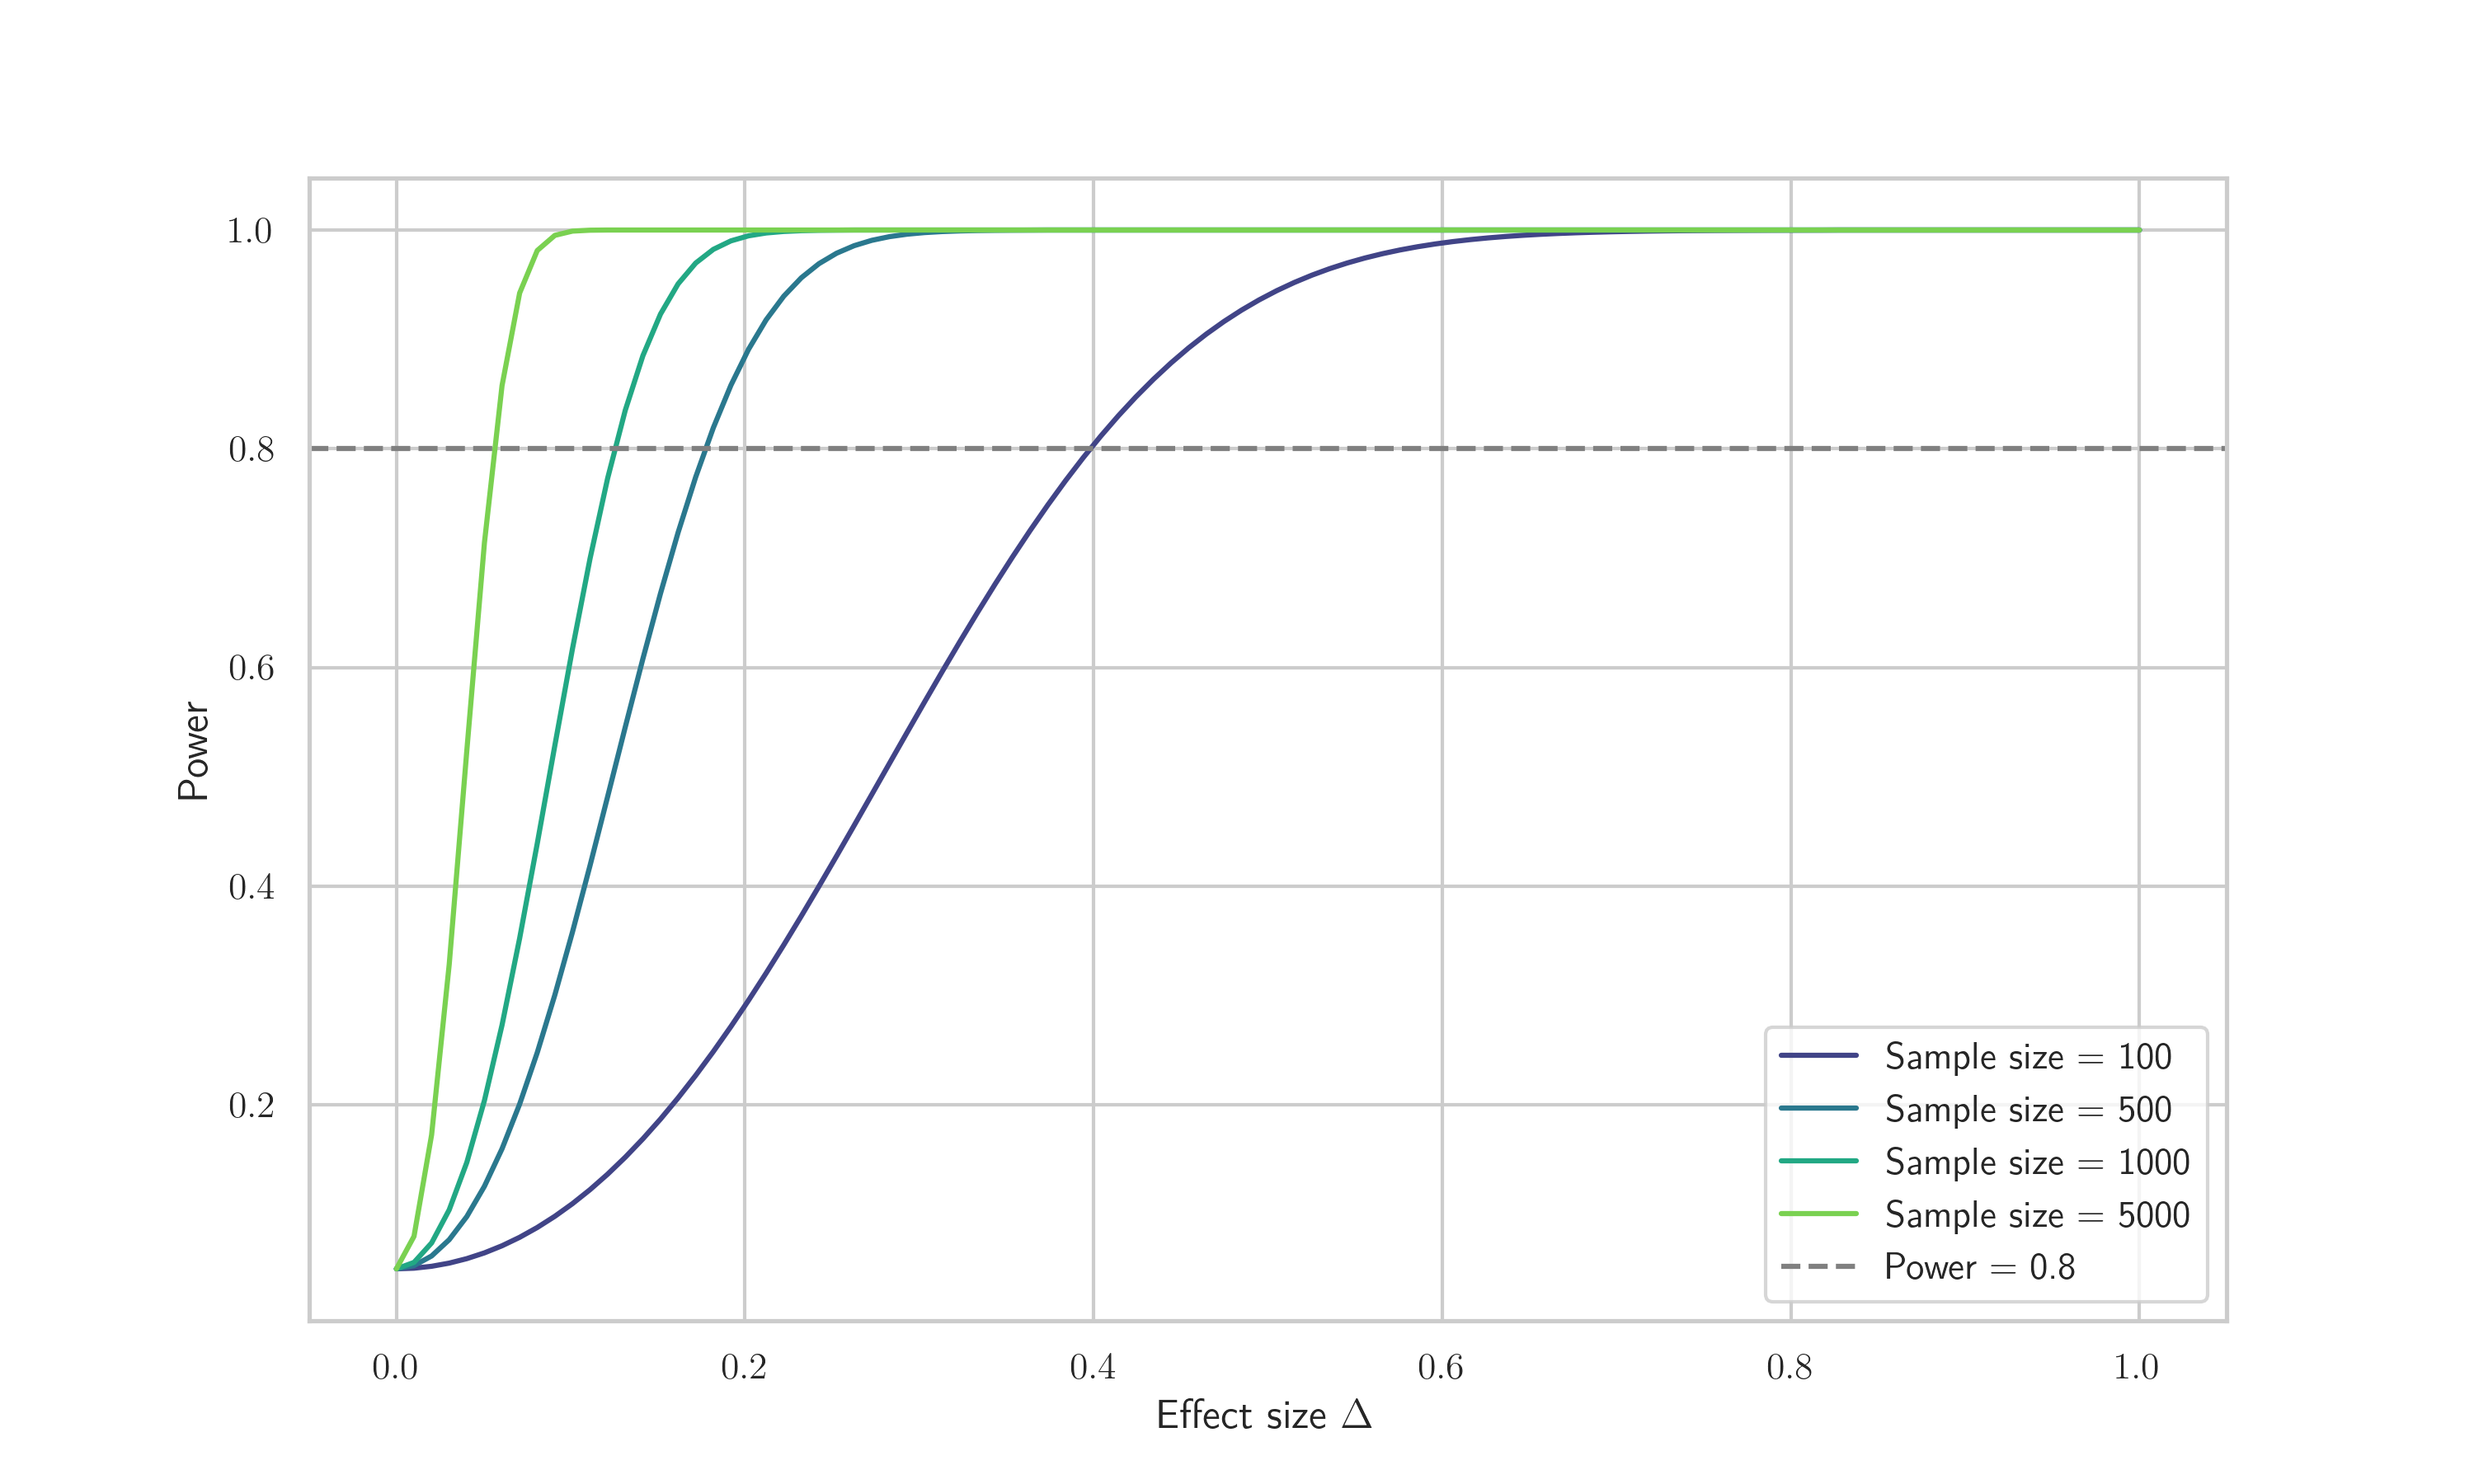
\includegraphics[width=\textwidth]{imagens/power_curve.png}
	\caption{Power curve for a two-sample t-test at significance level $\alpha = 0.05$. The curve illustrates the relationship between the effect size $\Delta$ and the power of the test for various sample sizes.}
	\label{fig:power_curve}
\end{figure}

This power curve demonstrates that to achieve a high probability of detecting a meaningful difference between the control and treatment groups, it is necessary to carefully consider both the sample size and the expected effect size. A well-designed A/B test balances these factors to ensure that the test is sufficiently powered while avoiding unnecessary increases in sample size \cite{Button2013}.
\subsection{Extensions and Variations in A/B Testing}

Classical A/B testing provides a robust framework for comparing two variants, but it can be extended to handle more complex experimental designs. One common extension is A/B/n testing, where more than two variants are compared simultaneously. In such cases, the risk of Type I errors increases due to multiple comparisons. To control the overall Type I error rate, adjustments such as the Bonferroni correction or the False Discovery Rate (FDR) control procedure are often applied \cite{Benjamini1995, Holm1979}.

Additionally, when the assumptions of normality or homoscedasticity (equal variances) are violated, non-parametric methods such as the Mann-Whitney U test or the Wilcoxon signed-rank test can be used as alternatives to the t-test. These methods are more robust to outliers and skewed distributions, providing reliable results even when the data do not meet the assumptions required for parametric tests \cite{Hollander2013}.

\subsubsection{Testing with Binary Random Variables}

In many A/B testing scenarios, the outcome of interest is binary, such as whether a user clicks on a link or not, whether a purchase is made, or whether a user subscribes to a service. When dealing with binary outcomes, the data can be modeled as coming from a Bernoulli distribution, where each observation takes the value 1 with probability $p$ (success) and 0 with probability $1-p$ (failure).

The classical two-sample t-test is not appropriate for binary data because the assumptions of normality and homoscedasticity are not met. Instead, other statistical tests are more suitable:

\paragraph{Chi-Square Test for Two Independent Groups:} The chi-square test is a statistical method used to determine whether there is a significant association between categorical variables across two independent groups. In A/B testing, it compares the distribution of binary outcomes (e.g., success vs. failure) between the control group (Group A) and the treatment group (Group B).

Let \(x_A\) and \(x_B\) represent the number of successes in Group A and Group B, respectively, with \(n_A\) and \(n_B\) being the corresponding total sample sizes for the two groups. The expected number of successes under the null hypothesis \(H_0\) (which assumes no association between group and outcome) is calculated as:

\[
E_A = \frac{(x_A + x_B) \cdot n_A}{n_A + n_B}, \quad E_B = \frac{(x_A + x_B) \cdot n_B}{n_A + n_B},
\]
where \(E_A\) and \(E_B\) are the expected numbers of successes in Groups A and B, respectively.

The chi-square statistic is then computed as:

\[
\chi^2 = \frac{(x_A - E_A)^2}{E_A} + \frac{(x_B - E_B)^2}{E_B} + \frac{(n_A - x_A - (n_A - E_A))^2}{n_A - E_A} + \frac{(n_B - x_B - (n_B - E_B))^2}{n_B - E_B},
\]
which follows a chi-square distribution with 1 degree of freedom under \(H_0\). This test helps determine if the observed difference in outcomes between the two groups is statistically significant \cite{Agresti2002}.



%\paragraph{Chi-Square Test for Two Independent Groups:} The chi-square test is a statistical method used to determine whether there is a significant association between categorical variables across two independent groups. In A/B testing, it compares the distribution of binary outcomes (e.g., success vs. failure) between the control group (Group A) and the treatment group (Group B).

%Given a 2x2 contingency table with observed frequencies \(O_{ij}\), where \(i\) represents the group and \(j\) represents the outcome, the expected frequencies \(E_{ij}\) under the null hypothesis \(H_0\) (which assumes no association between group and outcome) are calculated as:
%
%\[
%E_{ij} = \frac{O_{i\cdot} \cdot O_{\cdot j}}{N},
%\]
%where \(O_{i\cdot}\) and \(O_{\cdot j}\) are the marginal totals for the groups and outcomes, respectively, and \(N\) is the total sample size.
%
%The chi-square statistic is then computed as:
%
%\[
%\chi^2 = \sum_{i=1}^{2} \sum_{j=1}^{2} \frac{(O_{ij} - E_{ij})^2}{E_{ij}},
%\]
%which follows a chi-square distribution with 1 degree of freedom under \(H_0\). This test helps determine if the observed difference in outcomes between the two groups is statistically significant \cite{Agresti2002}.

\paragraph{Z-Test for Proportions:} When comparing two proportions, a Z-test for proportions can be used to test the null hypothesis that the proportions of successes in two independent groups are equal. The test statistic is given by:
\[
Z = \frac{\hat{p}_A - \hat{p}_B}{\sqrt{\hat{p}(1-\hat{p})\left(\frac{1}{n_A} + \frac{1}{n_B}\right)}},
\]
where $\hat{p}_A$ and $\hat{p}_B$ are the sample proportions for groups A and B, respectively, and $\hat{p}$ is the pooled proportion:
\[
\hat{p} = \frac{x_A + x_B}{n_A + n_B},
\]
with $x_A$ and $x_B$ being the number of successes in groups A and B, and $n_A$, $n_B$ are the respective sample sizes \cite{Newcombe1998}. The Z-test assumes that the sample sizes are large enough for the normal approximation to the binomial distribution to hold.

\paragraph{Logistic Regression:} For more complex analyses involving binary outcomes, logistic regression can be used to model the probability of success as a function of one or more predictor variables. In the context of A/B testing, logistic regression can model the relationship between the binary outcome and the group membership (A or B), while adjusting for other covariates. The model is given by:
\[
\text{logit}(p) = \log\left(\frac{p}{1-p}\right) = \beta_0 + \beta_1 \cdot X,
\]
where $p$ is the probability of success, $X$ is an indicator variable for group membership (1 for group B, 0 for group A), and $\beta_1$ represents the effect of the treatment \cite{Hosmer2013}. Logistic regression is particularly useful when dealing with multiple predictors and interactions.
\subsection{Conclusion}
%TODO ???
Classical A/B testing remains a cornerstone of experimental design, offering a straightforward and powerful method for comparing two variants. However, its effectiveness hinges on the correct implementation of the underlying statistical assumptions and careful consideration of practical challenges. As the field of A/B testing evolves, it is crucial for practitioners to stay vigilant about potential pitfalls, such as bias in randomization, inadequate sample sizes, and violations of test assumptions. By addressing these challenges, researchers can ensure that their experiments yield reliable and meaningful insights that can drive informed decision-making \cite{Kohavi2013}.

\section{Issues with Classical A/B Testing}

While classical A/B testing is a powerful and widely used methodology, it is not without its challenges and limitations. These issues primarily arise from the practical aspects of implementing A/B tests in dynamic, real-world environments, where the assumptions underlying the classical approach may not hold. This section discusses some of the key issues that can affect the validity and reliability of A/B test results.

\subsection{Peeking and Its Consequences}

One of the most prevalent pitfalls in classical A/B testing is the issue of "peeking," which refers to the practice of examining the data before the experiment is completed. The eagerness to make decisions based on early results often leads to peeking, especially in fast-paced environments where immediate results are highly valued. However, this practice can severely compromise the statistical integrity of the experiment by inflating the Type I error rate.

Mathematically, if an experimenter performs $k$ interim analyses during an ongoing experiment, each at a significance level $\alpha$, the cumulative probability of making at least one Type I error (rejecting a true null hypothesis) is approximately:
\[
\alpha_{\text{overall}} \approx 1 - (1 - \alpha)^k.
\]
For example, if $\alpha = 0.05$ and $k = 5$, the overall Type I error rate increases to about 0.226, meaning there is a 22.6\% chance of incorrectly rejecting the null hypothesis at least once during the experiment \cite{Pocock1977}.

To prevent this issue, researchers can employ several strategies:
\begin{itemize}
	\item \textbf{Fixed-Horizon Testing}: One of the simplest solutions is to set a fixed sample size or duration for the experiment and avoid looking at the data until the experiment concludes. This prevents premature decisions based on incomplete data.
	\item \textbf{Group Sequential Designs}: These designs allow for interim analyses at pre-specified points while controlling the overall Type I error rate. Such methods often employ stopping boundaries that determine whether the experiment should be stopped early for efficacy, futility, or if it should continue \cite{Pocock1977}.
	\item \textbf{Alpha Spending Functions}: This approach involves distributing the overall significance level $\alpha$ across multiple analyses in a way that maintains the desired error rate. The alpha spending function can be tailored to the specific needs of the study, allowing for more flexibility than traditional fixed designs \cite{DeMets1994}.
\end{itemize}

\subsection{Multiple Comparisons and False Discoveries}

Another critical issue in classical A/B testing is the challenge of multiple comparisons, which arises when multiple hypotheses are tested simultaneously or in quick succession. In such scenarios, the risk of encountering a false positive (Type I error) increases with each additional test conducted. This problem is particularly acute in large-scale A/B testing environments, such as those involving multiple variants of a product or feature.

To understand this mathematically, consider a situation where $m$ independent hypotheses are being tested, each at a significance level $\alpha$. The probability of at least one Type I error occurring among these tests can be controlled by adjusting the significance level for each individual test. A common approach is the Bonferroni correction, which adjusts the significance level to:
\[
\alpha^* = \frac{\alpha}{m}.
\]
While the Bonferroni correction is effective in controlling the family-wise error rate (FWER), it can be overly conservative, particularly when the number of tests $m$ is large, potentially leading to a loss of statistical power \cite{Holm1979}.

To address this, alternative methods such as the False Discovery Rate (FDR) control, introduced by Benjamini and Hochberg, offer a more balanced approach. FDR controls the expected proportion of Type I errors among the rejected hypotheses, rather than focusing on the occurrence of any Type I error. The Benjamini-Hochberg procedure orders the $p$-values from smallest to largest and determines the threshold for significance based on:
\[
p_{(k)} \leq \frac{k}{m} \alpha,
\]
where $p_{(k)}$ is the $k$-th smallest $p$-value. This method allows for a greater number of discoveries while maintaining control over the rate of false positives \cite{Benjamini1995}.

In more complex experimental setups, where decisions must be made dynamically, Pocock's group sequential methods can be adapted to allow for multiple analyses while controlling for the error rate across these analyses. These methods are particularly useful when tests are conducted sequentially, as they offer a structured approach to managing the cumulative risk of Type I errors \cite{Pocock1977}.

\subsection{Time-Varying Effects and External Influences}

Classical A/B testing assumes that the underlying conditions remain constant throughout the duration of the experiment. However, in real-world environments, this assumption is often violated. User behavior, market conditions, and external factors such as seasonality or competitive actions can change over time, introducing time-varying effects that can bias the results.

Consider an A/B test conducted over several weeks, where user engagement might be influenced by external events, such as holidays or news cycles. If these external factors affect one group differently than the other, the assumption of independence between groups is violated, leading to biased estimates of the treatment effect \cite{Rosenbaum2010}.

To address these issues, several approaches can be considered:
\begin{itemize}
	\item \textbf{Time-Series Analysis}: Techniques such as time-series regression or autoregressive integrated moving average (ARIMA) models can help account for time-varying effects and autocorrelation in the data. This allows for a more accurate estimation of the treatment effect, accounting for trends and seasonal variations \cite{Box2015}.
	\item \textbf{Adaptive Experimentation}: Adaptive experimental designs, such as multi-armed bandit algorithms, can adjust the allocation of subjects to different groups in real-time based on observed performance. This approach is particularly useful in dynamic environments, where the conditions affecting user behavior can change rapidly \cite{Scott2015}.
	\item \textbf{Randomization Over Time}: By randomizing the exposure to different variations over time, rather than all at once, it is possible to reduce the impact of time-varying effects. This approach, known as temporal randomization, can help ensure that each variation is exposed to a representative sample of users across different time periods, reducing the risk of bias due to external influences \cite{Montgomery2008}.
\end{itemize}

\subsection{Conclusion}
%TODO
While classical A/B testing remains a valuable tool for experimentation, it is important to be aware of the potential pitfalls and limitations associated with its use. Issues such as peeking, multiple comparisons, and time-varying effects can significantly impact the validity of the results if not properly addressed. By employing appropriate statistical methods and adhering to best practices in experimental design, researchers and practitioners can mitigate these risks and ensure more reliable and accurate outcomes.

\section{Theoretical Foundations: Game Theory and Decision Functions}

This section introduces the foundational concepts of game theory and decision functions, both of which are essential for understanding and optimizing A/B testing. We will first delve into game theory, exploring how strategic interactions between decision-makers can influence experimental outcomes, followed by a detailed discussion on decision functions in statistical decision theory.


\subsection{Game Theory}

Game theory is the study of strategic interactions among rational decision-makers, where the outcome for each participant depends not only on their own actions but also on the actions of others. This framework is crucial for analyzing scenarios where multiple stakeholders or users interact in a shared environment, such as in A/B testing.

\subsubsection{Fundamental Concepts in Game Theory}

Game theory is built on several foundational concepts:

\begin{definition}[Players]
	In game theory, the decision-makers involved in the interaction are referred to as \textbf{players}. Each player aims to maximize their own payoff, which depends on the strategies chosen by all players. In A/B testing, players can represent different teams within an organization (e.g., marketing, product development) or the users who interact with the variants being tested.
\end{definition}

\begin{definition}[Strategies]
	A \textbf{strategy} is a complete plan of action that a player follows throughout the game. The set of all possible strategies available to a player is known as the \textbf{strategy space}. In A/B testing, strategies might include decisions on the sample size, timing of interim analyses, stopping criteria, or even how users interact with different variants.
\end{definition}

\begin{definition}[Payoffs]
	 The \textbf{payoff} is the reward or outcome that a player receives based on the combination of strategies chosen by all players. The payoff function \( u_i(s_1, s_2, \dots, s_n) \) assigns a numerical value to the outcome for player \( i \) given the strategy profile \( (s_1, s_2, \dots, s_n) \). In A/B testing, payoffs could be metrics such as conversion rates, revenue, or user engagement.
\end{definition}



\begin{definition}[Games in Strategic Form]
	A game in \textbf{strategic form} (or normal form) is defined by:
	\begin{itemize}
		\item The set of players \( N = \{1, 2, \dots, n\} \).
		\item The strategy space \( S_i \) for each player \( i \).
		\item The payoff function \( u_i: S_1 \times S_2 \times \dots \times S_n \rightarrow \mathbb{R} \) for each player \( i \).
	\end{itemize}
	The strategic form captures the essential elements of the game, facilitating the analysis of optimal strategies and equilibria.
\end{definition}


\begin{definition}[Nash Equilibrium]
	A \textbf{Nash equilibrium} is a strategy profile \( (s_1^*, s_2^*, \dots, s_n^*) \) where no player can improve their payoff by unilaterally changing their strategy:
	\[
	u_i(s_1^*, s_2^*, \dots, s_i^*, \dots, s_n^*) \geq u_i(s_1^*, s_2^*, \dots, s_i, \dots, s_n^*),
	\]
	for all \( i \) and for all alternative strategies \( s_i \). The Nash equilibrium represents a stable outcome where each player's strategy is the best response to the strategies of the other players \cite{Nash1951}.
\end{definition}

\subsubsection{Types of Games and Their Application to A/B Testing}

Game theory encompasses various types of games, each with unique characteristics and applications to A/B testing:

\paragraph{Cooperative vs. Non-Cooperative Games}

In \textbf{cooperative games}, players can form binding agreements and collaborate to achieve a better outcome. In contrast, \textbf{non-cooperative games} focus on strategic interactions where each player acts independently to maximize their own payoff without binding agreements. Most A/B testing scenarios are modeled as non-cooperative games, where different teams or users act independently, pursuing their own objectives.

\paragraph{Static vs. Dynamic Games}

In \textbf{static games}, all players choose their strategies simultaneously, with no knowledge of the other players' choices. In \textbf{dynamic games}, players make decisions sequentially, with some players observing the earlier actions of others. Dynamic games are particularly relevant in A/B testing when decisions are made in stages, such as during interim analyses or when adapting the experiment based on preliminary results.

\paragraph{Complete vs. Incomplete Information Games}

In games of \textbf{complete information}, all players know the payoff functions and strategies available to all other players. In \textbf{incomplete information games}, players have private information, such as their own payoff function or the probability distribution of other players' payoffs. Incomplete information games are common in A/B testing, where different stakeholders may have private information about user preferences or the expected impact of the variants. \textbf{Bayesian games} are a type of incomplete information game where players have beliefs about the types of other players, represented by probability distributions \cite{Harsanyi1967}.

\subsubsection{Advanced Concepts in Game Theory Applied to A/B Testing}

Beyond the basic game-theoretic concepts, several advanced ideas are particularly relevant to A/B testing:

\begin{definition}[Mixed Strategy]
	A \textbf{mixed strategy} is a probability distribution over a player's pure strategies. Instead of choosing a single strategy with certainty, a player randomizes over available strategies. A \textbf{mixed strategy Nash equilibrium} occurs when each player's mixed strategy is the best response to the mixed strategies of the other players.
\end{definition}

In A/B testing, mixed strategies could be used when deploying variants probabilistically rather than deterministically. This approach can help balance exploration and exploitation, especially in uncertain environments \cite{Aumann1974}.


\begin{definition}[Correlated Equilibria]
	A \textbf{correlated equilibrium} is a generalization of the Nash equilibrium, where players may coordinate their strategies based on signals from a correlation device. This concept allows for more flexible strategic interactions and can lead to outcomes where all players achieve higher payoffs compared to a Nash equilibrium.
\end{definition}

Correlated equilibria are relevant in A/B testing when there is an external signal or trend (e.g., a seasonal effect or market shift) that all stakeholders can observe and use to coordinate their strategies \cite{Aumann1987}.


\begin{definition}[Repeated Games]
	\textbf{Repeated games} involve the same players playing a game multiple times. The strategies in repeated games can depend on the history of play, allowing for more complex strategic interactions, such as cooperation, punishment, and reputation-building.
\end{definition}

In A/B testing, repeated games can model situations where the same test or similar tests are conducted multiple times, and the decisions in one test influence future tests. Repeated games can help in understanding how long-term strategies evolve and how cooperation or competition between teams might develop over time \cite{Fudenberg1991}.

\begin{definition}[Multi-Armed Bandit Problems]
	The \textbf{multi-armed bandit problem} is a classic problem in game theory that involves allocating resources among competing options (or "arms") to maximize cumulative rewards. In A/B testing, this translates to dynamically allocating users to different variants based on the performance of those variants.
\end{definition}

The challenge is to balance exploration (gathering information about the effectiveness of each variant) with exploitation (using the best-known variant to maximize rewards). Solutions to the multi-armed bandit problem, such as \textbf{Thompson Sampling} or the \textbf{Upper Confidence Bound (UCB)} algorithm, are commonly used in adaptive A/B testing to optimize the allocation of traffic among variants \cite{Lai1985}.

\subsubsection{Application of Game Theory to Real-World A/B Testing Scenarios}

Game theory provides valuable insights into several practical aspects of A/B testing:

\paragraph{Stakeholder Interaction and Conflict Resolution}

Different teams involved in A/B testing may have conflicting objectives. For instance, the marketing team might prioritize short-term engagement metrics, while the product development team focuses on long-term user retention. Game theory can model these interactions and help identify strategies that lead to a Nash equilibrium, where all stakeholders are satisfied with the outcome.

Game theory can also be used to design mechanisms that incentivize cooperation between teams, ensuring that the chosen variant balances the interests of all parties. For example, introducing a correlation device (as in correlated equilibria) might allow teams to coordinate their strategies based on shared information, leading to a more efficient and equitable outcome.

\paragraph{User Behavior and Strategic Interaction}

Users in an A/B test are not passive participants; their behavior can influence the outcome of the test. For instance, users might adapt to changes in the user interface, or their behavior might change based on their perceptions of the different variants. Game theory provides a framework for anticipating such strategic behavior and designing tests that account for these interactions.

By modeling the users as players in a game, experimenters can predict how different test designs might influence user behavior and adjust their strategies accordingly. This approach is particularly important in online experiments, where user behavior can have a significant impact on the validity of the test results.

\paragraph{Dynamic and Adaptive Testing Strategies}

Game theory is also applicable in the design of dynamic and adaptive A/B testing strategies. For example, in a dynamic game, the experimenters might decide whether to continue the test, stop it early, or switch to a different variant based on the data collected so far. This decision-making process can be modeled as a sequential game, where each stage of the test represents a move in the game.

Adaptive testing strategies, such as those used in multi-armed bandit problems, can also be analyzed using game theory. These strategies dynamically allocate users to different variants based on their performance, optimizing the test outcome over time. Game theory provides the tools to understand the trade-offs between exploration and exploitation in these adaptive strategies and to design tests that achieve the desired balance.


\subsection{Conclusion}
%TODO
Game theory offers a rich and powerful framework for analyzing the strategic interactions that occur in A/B testing. By modeling the decisions of different stakeholders and users as a game, experimenters can gain deeper insights into how these interactions influence the outcome of the test. Game theory not only helps in identifying optimal strategies and equilibria but also provides a foundation for designing tests that are robust to strategic behavior and capable of balancing competing objectives.

In the context of A/B testing, game theory enhances our understanding of how to navigate complex decision-making environments, anticipate user behavior, and design experiments that lead to reliable and actionable results. As A/B testing continues to evolve, the application of game theory will become increasingly important in ensuring that tests are both scientifically rigorous and strategically sound.
\subsection{Decision Functions in Statistical Decision Theory}

In statistical decision theory, decision functions are the mathematical tools used to make optimal decisions under uncertainty. A decision function maps the observed data to an action, guiding the decision-making process in a way that minimizes potential losses or maximizes expected gains. This subsection explores the foundational concepts, criteria for optimality, and specific examples of decision functions, particularly in the context of A/B testing.

\subsubsection{Basic Definitions and Concepts}

Consider a decision-making scenario where the true state of nature is represented by a parameter \( \theta \in \Theta \), with \( \Theta \) being the parameter space. The decision-maker observes data \( X \in \mathcal{X} \), where \( \mathcal{X} \) is the sample space, and must choose an action \( a \in \mathcal{A} \), where \( \mathcal{A} \) is the action space.
\begin{definition}[Decision Functio]
	A \textbf{decision function} \( \delta: \mathcal{X} \rightarrow \mathcal{A} \) is a rule that prescribes an action based on the observed data \( X \). 
\end{definition}
The goal of a decision function is to make choices that optimize the expected outcome, given thex uncertainty about the true state of nature \( \theta \).

\begin{definition}[Loss Function]
	The quality of a decision is evaluated using a \textbf{loss function} \( L(\theta, a) \), which quantifies the cost associated with choosing action \( a \) when the true state is \( \theta \).
\end{definition}
The loss function is central to decision theory, as it reflects the consequences of decisions under different scenarios.

\begin{definition}[Risk Function]
	The \textbf{risk function} \( R(\theta, \delta) \) represents the expected loss associated with the decision function \( \delta \) for a given parameter \( \theta \):
	\[
	R(\theta, \delta) = \mathbb{E}_{X \mid \theta}[L(\theta, \delta(X))] = \int_{\mathcal{X}} L(\theta, \delta(x)) \, p(x \mid \theta) \, dx,
	\]
	where \( p(x \mid \theta) \) is the probability density function of \( X \) given \( \theta \). 
\end{definition}
The risk function provides a measure of the performance of a decision function over different possible states of nature.

\subsubsection{Optimality Criteria in Decision Functions}

Several criteria are used to evaluate and select decision functions, each reflecting different approaches to risk and uncertainty:

\begin{definition}[Bayes Criterion]
	The \textbf{Bayes criterion} incorporates prior knowledge about the parameter \( \theta \) through a prior distribution \( \pi(\theta) \). The Bayes risk is the expected value of the risk function with respect to this prior:
	\[
	r(\pi, \delta) = \int_{\Theta} R(\theta, \delta) \, \pi(\theta) \, d\theta.
	\]
\end{definition}
	
\begin{definition}[Bayes decision function]
	The decision function \( \delta^* \) that minimizes the Bayes risk is known as the \textbf{Bayes decision function}:
	\[
	\delta^*(x) = \arg \min_{a \in \mathcal{A}} \int_{\Theta} L(\theta, a) \, \pi(\theta \mid x) \, d\theta,
	\]
	where \( \pi(\theta \mid x) \) is the posterior distribution of \( \theta \) given the observed data \( x \).
\end{definition}



The Bayes criterion is particularly useful when reliable prior information about \( \theta \) is available, as it allows the decision-maker to update their beliefs and make informed decisions based on both prior knowledge and observed data \cite{Berger1985}.

\begin{definition}[Minimax Criterion]
	The \textbf{minimax criterion} provides a robust approach to decision-making in the absence of reliable prior information. It focuses on minimizing the maximum possible risk:
	\[
	\delta^* = \arg \min_{\delta} \max_{\theta \in \Theta} R(\theta, \delta).
	\]
\end{definition}

This criterion is conservative, ensuring that the decision function performs well even in the worst-case scenario. The minimax decision rule is often employed in situations with high uncertainty or when the consequences of making an incorrect decision are severe \cite{Wald1950}.

\begin{definition}[Admissibility and Dominance]
	
	In statistical decision theory, a decision function \( \delta: \mathcal{X} \rightarrow \mathcal{A} \) is considered \textbf{admissible} if there does not exist another decision function \( \delta': \mathcal{X} \rightarrow \mathcal{A} \) that dominates it. This is formally expressed as:
	\[
	R(\theta, \delta') \leq R(\theta, \delta) \quad \text{for all } \theta \in \Theta,
	\]
	with strict inequality for some \( \theta_0 \in \Theta \), meaning:
	\[
	R(\theta_0, \delta') < R(\theta_0, \delta).
	\]
\end{definition}

In other words, if a decision function \( \delta' \) exists such that it yields a lower or equal risk for every possible state of nature \( \theta \), and strictly lower risk for at least one \( \theta_0 \), then \( \delta \) is deemed \textbf{inadmissible}. An inadmissible decision function can be improved upon by switching to \( \delta' \), which offers a strictly better performance in at least one scenario without worsening it in others.

Admissibility is crucial in decision theory as it eliminates suboptimal decision functions. An admissible decision function cannot be universally improved upon, making it a candidate for optimality under various criteria. The concept of admissibility ensures that the chosen decision function performs well across all possible scenarios, making it a robust choice in uncertain environments \cite{Lehmann1998}.

\begin{definition}[Pareto Optimality]
	In multi-objective decision-making scenarios, the concept of \textbf{Pareto optimality} is used to evaluate decision functions. A decision function is Pareto optimal if there is no other function that improves one objective without worsening another. Formally, \( \delta \) is Pareto optimal if there does not exist a \( \delta' \) such that:
	\[
	R_i(\theta, \delta') \leq R_i(\theta, \delta) \quad \text{for all } i,
	\]
	with strict inequality for at least one \( i \), where \( R_i(\theta, \delta) \) represents the risk associated with the \( i \)-th objective.
\end{definition}


Pareto optimality is particularly relevant in A/B testing when balancing the interests of multiple stakeholders, such as marketing, product development, and user experience teams. It ensures that the chosen decision function achieves a balanced trade-off between competing objectives \cite{Miettinen1999}.

\subsubsection{Examples of Decision Functions in A/B Testing}

In the context of A/B testing, decision functions guide the experimenter in determining whether to adopt a new variant (B) over a control (A) based on the observed data. Several common decision functions include:

\begin{example}[Threshold-Based Decision Function]
	One simple decision function is to reject the null hypothesis \( H_0 \) (that there is no difference between A and B) if the test statistic \( T(X) \) exceeds a critical value \( c \):
	\[
	\delta(X) = 
	\begin{cases} 
		\text{Adopt B} & \text{if } T(X) > c, \\
		\text{Retain A} & \text{otherwise}.
	\end{cases}
	\]
\end{example}

Here, the loss function may reflect the cost of adopting a suboptimal variant, and the risk function quantifies the expected loss under different scenarios, such as false positives (Type I errors) or false negatives (Type II errors).

\begin{example}[Bayesian Decision Function]

In a Bayesian framework, the decision to adopt variant B over A is based on the posterior probability that B is better than A, given the observed data. Let \( \pi(\theta_B > \theta_A \mid X) \) represent this posterior probability. A Bayesian decision function is defined by comparing this posterior probability against a pre-specified threshold \( \gamma \) that reflects the decision-maker's tolerance for risk and uncertainty:
\[
\delta(X) = 
\begin{cases} 
	\text{Adopt B} & \text{if } \pi(\theta_B > \theta_A \mid X) > \gamma, \\
	\text{Retain A} & \text{otherwise}.
\end{cases}
\]
\end{example}

The threshold \( \gamma \) is typically chosen based on the decision-maker's preferences, with higher values of \( \gamma \) indicating a more conservative approach (i.e., requiring stronger evidence to adopt the new variant B). This decision function directly incorporates prior knowledge and updates it based on the observed data, allowing for decisions that are informed by both the prior beliefs and the current evidence.

By adjusting \( \gamma \), the decision-maker can control the balance between Type I errors (false positives) and Type II errors (false negatives), tailoring the decision process to the specific needs and risk tolerance of the experiment.

\begin{example}[Sequential Decision Function]
	In sequential A/B testing, the decision function might involve continuous monitoring of the data and stopping the test as soon as sufficient evidence is gathered. For example, a sequential decision function could be:
	\[
	\delta(X) = 
	\begin{cases} 
		\text{Stop and adopt B} & \text{if } T_n > c, \\
		\text{Stop and retain A} & \text{if } T_n < -c, \\
		\text{Continue testing} & \text{otherwise},
	\end{cases}
	\]
	where \( T_n \) is the test statistic after \( n \) observations, and \( c \) is a pre-specified threshold.
\end{example}
 Sequential decision functions are particularly effective in reducing the required sample size, as the test can be stopped early if there is strong evidence for one variant over the other \cite{Wald1947}.

\subsubsection{Decision Functions in the Context of Loss Functions}

The choice of a decision function is closely related to the choice of a loss function, as different loss functions lead to different optimal decision rules. Common types of loss functions include:

\begin{example}[Binary Loss Function]
	The \textbf{binary loss function} is a simple binary loss function used in hypothesis testing, where:
	\[
	L(\theta, a) = 
	\begin{cases} 
		0 & \text{if the correct decision is made}, \\
		1 & \text{if the incorrect decision is made}.
	\end{cases}
	\]
\end{example}

This loss function is often used in binary classification problems and hypothesis testing, where the goal is to minimize the probability of making an incorrect decision.

\begin{example}[Quadratic Loss Function]
The \textbf{quadratic loss function} penalizes errors based on the square of the difference between the estimated and true parameter values:
\[
L(\theta, a) = (\theta - a)^2.
\]
\end{example}

This loss function is common in estimation problems, where it encourages decisions that minimize the mean squared error. In A/B testing, it might be used when the goal is to minimize the squared difference between the observed effect size and the true effect size.

\begin{example}[Asymmetric Loss Function]
	In some cases, the cost of different types of errors is not symmetric. For instance, in A/B testing, the cost of adopting a suboptimal variant might be higher than the cost of missing a small improvement. An \textbf{asymmetric loss function} reflects this by assigning different penalties to different types of errors:
	\[
	L(\theta, a) = 
	\begin{cases} 
		\lambda_1(\theta - a) & \text{if } \theta > a, \\
		\lambda_2(a - \theta) & \text{if } \theta \leq a,
	\end{cases}
	\]
	where \( \lambda_1 \) and \( \lambda_2 \) are different penalty coefficients.
\end{example}

 This type of loss function can lead to decision functions that are more conservative or aggressive, depending on the relative costs of the errors.

\subsection{Conclusion}
%TODO
Decision functions are fundamental to the application of statistical decision theory in A/B testing. They provide a structured approach to making optimal decisions based on observed data, balancing different objectives and uncertainties. By formalizing the decision-making process through decision functions, experimenters can ensure that their choices are statistically justified and aligned with the overall goals of the test.

In A/B testing, decision functions are essential for determining when to stop the test, which variant to adopt, and how to balance competing interests and uncertainties. The choice of an appropriate decision function depends on the specific context of the test, including the available prior information, the nature of the loss function, and the desired balance between different types of errors.


\section{Sequential A/B Testing Methods}

Sequential A/B testing represents an advanced methodology that enhances traditional A/B testing by allowing for continuous data evaluation and adaptive decision-making. Unlike classical A/B testing, which relies on a fixed sample size and makes decisions only after all data is collected, sequential A/B testing evaluates data as it is accumulated. This approach can lead to earlier conclusions, more efficient use of resources, and ethical advantages, particularly in situations where prolonged exposure to inferior treatments or variants is undesirable.

\subsection{Theoretical Foundations of Sequential A/B Testing}

Sequential A/B testing is grounded in the principles of sequential analysis, which permits hypothesis testing as data accumulates rather than requiring a fixed sample size. This method is particularly advantageous in scenarios where early decision-making is crucial, such as in online experiments or clinical trials, where rapid iteration or ethical considerations are paramount.

\subsubsection{Hypothesis Formulation}
%TODO zmeinc forme testu
As with traditional A/B testing, the first step in sequential A/B testing is to define the null and alternative hypotheses. The null hypothesis \( H_0 \) posits that there is no difference in the mean outcomes between the two variants, while the alternative hypothesis \( H_1 \) suggests a difference:
\begin{align*}
	H_0 &: \mu_A = \mu_B, \\
	H_1 &: \mu_A \neq \mu_B.
\end{align*}
where \( \mu_A \) and \( \mu_B \) represent the expected values of the performance metric (such as conversion rates) for the control (A) and treatment (B) groups, respectively. The objective of the sequential A/B test is to decide whether to accept \( H_0 \) or \( H_1 \) based on the data collected up to a certain point, with the flexibility to stop the test as soon as sufficient evidence is gathered.

\subsubsection{Sequential Probability Ratio Test (SPRT)}

The Sequential Probability Ratio Test (SPRT), developed by Abraham Wald, is the cornerstone of sequential analysis and is widely applicable to A/B testing. SPRT provides a systematic method for continuously evaluating the evidence in favor of \( H_0 \) or \( H_1 \) as data is collected.

\paragraph{Likelihood Ratio}

At each stage \( n \) of data collection, the likelihood ratio \( \Lambda_n \) is calculated as:

\[
\Lambda_n = \frac{\prod_{i=1}^{n} f(X_i; \theta_1)}{\prod_{i=1}^{n} f(X_i; \theta_0)},
\]

where \( f(X_i; \theta) \) is the probability density function (or probability mass function in the case of discrete data) of the observation \( X_i \) under the parameter \( \theta \). For A/B testing, \( \theta_0 \) and \( \theta_1 \) represent the parameters under the null and alternative hypotheses, respectively.

Alternatively, the log-likelihood ratio \( \log \Lambda_n \) can be expressed as:

\[
\log \Lambda_n = \sum_{i=1}^{n} \log \left(\frac{f(X_i; \theta_1)}{f(X_i; \theta_0)}\right),
\]

which accumulates evidence for or against \( H_0 \) as data is observed. The decision at stage \( n \) is then based on this accumulated evidence.

\paragraph{Decision Rule}

The decision to continue, stop, or reject the null hypothesis in SPRT is based on comparing the likelihood ratio \( \Lambda_n \) to two predefined thresholds \( A \) and \( B \):

\begin{align*}
	\text{If } \Lambda_n &\geq B, \quad \text{reject } H_0 \text{ in favor of } H_1, \\
	\text{If } \Lambda_n &\leq A, \quad \text{accept } H_0 \text{ and stop the test}, \\
	\text{If } A < \Lambda_n &< B, \quad \text{continue collecting data}.
\end{align*}

The thresholds \( A \) and \( B \) are chosen to control the Type I error rate \( \alpha \) and the Type II error rate \( \beta \):

\[
A = \frac{1 - \beta}{\alpha}, \quad B = \frac{\beta}{1 - \alpha}.
\]

These thresholds ensure that the test maintains the desired error rates while allowing for early stopping if sufficient evidence accumulates.

\paragraph{Expected Sample Size}
%TODO nie wiem czy nei usunąć
The efficiency of the SPRT is reflected in its ability to minimize the expected sample size \( E(n) \). Under the assumptions of the test, the expected sample size required to reach a decision is often significantly smaller than that required by a fixed-sample test with the same error rates. 

\begin{theorem}
The expected sample size \( E(n) \) can be approximated using Wald's approximation:
\[
E(n) \approx \frac{\log B - \log A}{I(\theta_0, \theta_1)},
\]
where \( I(\theta_0, \theta_1) \) is the Kullback-Leibler information number, defined as:

\[
I(\theta_0, \theta_1) = \mathbb{E}_{\theta_1}\left[\log \left(\frac{f(X; \theta_1)}{f(X; \theta_0)}\right)\right].
\]
\end{theorem}

This information measure quantifies the expected log-likelihood ratio under the alternative hypothesis and directly influences the efficiency of the SPRT.

\subsubsection{Mixture Sequential Probability Ratio Test (mSPRT)}

The Mixture Sequential Probability Ratio Test (mSPRT) extends the classical SPRT to handle cases where the alternative hypothesis is not a single point but a range of possible values. This approach is particularly useful in practical A/B testing scenarios where the effect size between the control and treatment groups is uncertain.

\paragraph{Mixture Likelihood Ratio}

In mSPRT, instead of testing against a fixed alternative \( \theta_1 \), the test considers a mixture of possible alternatives \( \Theta_1 \). The likelihood ratio is then modified to integrate over this range:

\[
\Lambda_n = \frac{\int_{\Theta_1} w(\theta) \prod_{i=1}^{n} f(X_i; \theta) \, d\theta}{\prod_{i=1}^{n} f(X_i; \theta_0)},
\]

where \( w(\theta) \) is a weighting function that reflects prior beliefs about the distribution of \( \theta \) within the space \( \Theta_1 \). This mixture approach allows the test to be more robust against uncertainty in the effect size, providing greater flexibility and adaptability in practical A/B testing applications.

\paragraph{Decision Rule}

The decision-making process in mSPRT follows the same structure as in SPRT but applies to the mixture likelihood ratio \( \Lambda_n \):

\begin{align*}
	\text{If } \Lambda_n &\geq B, \quad \text{reject } H_0 \text{ in favor of } H_1, \\
	\text{If } \Lambda_n &\leq A, \quad \text{accept } H_0 \text{ and stop the test}, \\
	\text{If } A < \Lambda_n &< B, \quad \text{continue collecting data}.
\end{align*}

By considering a range of plausible effect sizes, mSPRT enhances the robustness of the decision-making process, particularly in environments where the effect size is uncertain or variable.

\paragraph{Bayesian Connection}

There is a natural connection between mSPRT and Bayesian methods, as the weighting function \( w(\theta) \) can be interpreted as a prior distribution over the parameter space \( \Theta_1 \). This Bayesian interpretation allows for a seamless integration of prior knowledge into the sequential testing framework, enhancing the flexibility and adaptability of the method.

\paragraph{Visualization: Likelihood Surface of mSPRT}
%TODO nie wiem czy nie usunac
A potential visualization could involve plotting the likelihood surface across the parameter space \( \Theta_1 \). This 3D plot or contour map would depict how the mixture likelihood ratio evolves as data accumulates, illustrating the test's ability to account for uncertainty in the effect size.

\subsubsection{Stopping Rules and Error Control}

A key feature of sequential A/B testing is the implementation of stopping rules, which determine when the test should conclude. The stopping rule \( \tau \) is a random variable representing the time (or number of observations) at which the test stops. The stopping rule is crucial for controlling the overall error rates \( \alpha \) and \( \beta \), ensuring that the sequential nature of the test does not inflate these rates.
\paragraph{Theoretical Foundations}

Consider a scenario where we have paired data \((x_i, y_i)\) for \(i = 1, 2, \dots, t\), where \(x_i\) and \(y_i\) represent the outcomes from two different populations or treatments (e.g., control and treatment groups in an A/B test). The goal is to test the hypothesis \(H: \theta_1 \leq \theta_2\), where \(\theta_1\) and \(\theta_2\) are parameters of interest (e.g., means or proportions) for the two populations.

Girshick's test reformulates the SPRT for this paired data context by defining two specific hypotheses:
\begin{align*}
	H_0: &\quad \theta_1 = \theta_0^1 \quad \text{and} \quad \theta_2 = \theta_0^2, \\
	H_1: &\quad \theta_1 = \theta_0^2 \quad \text{and} \quad \theta_2 = \theta_0^1.
\end{align*}
where \(\theta_0^1\) and \(\theta_0^2\) represent specific values that define the magnitude of difference deemed important for business decisions.

\begin{example}[Normally Distributed Data with Equal Variances and Different Means]
	
	
	Consider the case where the observations \(x_i\) and \(y_i\) are normally distributed with the same variance \(\sigma^2\), but different means \(\mu_1 = \theta_1\) and \(\mu_2 = \theta_2\). The data can be modeled as:
	\begin{align*}
		x_i &\sim \mathcal{N}(\theta_1, \sigma^2), \\
		y_i &\sim \mathcal{N}(\theta_2, \sigma^2),
	\end{align*}
	where \(\mathcal{N}(\mu, \sigma^2)\) denotes a normal distribution with mean \(\mu\) and variance \(\sigma^2\).
	The probability ratio test statistic after \(t\) pairs of data is given by:
	\begin{align*}
		\frac{p_1^t}{p_0^t} &= \prod_{i=1}^{t} \frac{f_{\theta_0^2}(x_i) f_{\theta_0^1}(y_i)}{f_{\theta_0^1}(x_i) f_{\theta_0^2}(y_i)}.
	\end{align*}
	%TODO w dodatku dowód
	This can be simplified to:
	\begin{align*}
		\frac{p_1^t}{p_0^t} &= \exp\left(\frac{\theta_0^2 - \theta_0^1}{\sigma^2} \cdot \sum_{i=1}^{t} (x_i - y_i)\right).
	\end{align*}
	
	Taking the logarithm, the log-likelihood ratio becomes:
	\begin{align*}
		\log \left(\frac{p_1^t}{p_0^t}\right) &= \frac{\theta_0^2 - \theta_0^1}{\sigma^2} \cdot \sum_{i=1}^{t} (x_i - y_i).
	\end{align*}
	
	This log-likelihood ratio can be used to make decisions at each stage of data collection, where the test will continue until the log-likelihood ratio exceeds a certain threshold, indicating sufficient evidence to reject the null hypothesis.
\end{example}

\begin{example}[Bernoulli Distributed Data with Different Success Probabilities]
	Now, consider the case where the outcomes \(x_i\) and \(y_i\) are Bernoulli distributed with success probabilities \(\theta_1 = p_1\) and \(\theta_2 = p_2\), respectively. The data can be modeled as:
	\begin{align*}
		x_i &\sim \text{Bernoulli}(\theta_1), \\
		y_i &\sim \text{Bernoulli}(\theta_2),
	\end{align*}
	where \(\text{Bernoulli}(p)\) denotes a Bernoulli distribution with success probability \(p\).
	
	The probability ratio test statistic after \(t\) pairs of data is given by:
	\begin{align*}
		\frac{p_1^t}{p_0^t} = \prod_{i=1}^{t} \frac{{\theta_0^2}^{x_i}(1-\theta_0^2)^{1-x_i} \cdot {\theta_0^1}^{y_i}(1-\theta_0^1)^{1-y_i}}{{\theta_0^1}^{x_i}(1-\theta_0^1)^{1-x_i} \cdot {\theta_0^2}^{y_i}(1-\theta_0^2)^{1-y_i}}.
	\end{align*}
	
	This simplifies to:
	\begin{align*}
		\frac{p_1^t}{p_0^t} &= \left(\frac{\theta_0^2(1-\theta_0^1)}{\theta_0^1(1-\theta_0^2)}\right)^{\sum_{i=1}^{t} (x_i - y_i)}.
	\end{align*}
	
	Taking the logarithm, the log-likelihood ratio becomes:
	\begin{align*}
		\log \left(\frac{p_1^t}{p_0^t}\right) &= \sum_{i=1}^{t} (y_i - x_i) \cdot \log \left(\frac{\theta_0^1(1-\theta_0^2)}{\theta_0^2(1-\theta_0^1)}\right).
	\end{align*}
	
	Again, this log-likelihood ratio is used to evaluate the evidence in favor of the alternative hypothesis \(H_1\) as data is collected.
\end{example}

\begin{lemma}[Deviance Measure For Bernoulli Distribution]
	The deviance measure \(\nu(\theta_1, \theta_2)\) for Bernoulli distributions is given by:
	\begin{align*}
		\nu(\theta_1, \theta_2) &= \log \left(\frac{1 - \theta_2}{1 - \theta_1} \cdot \frac{\theta_1}{\theta_2}\right).
	\end{align*}
\end{lemma}

\begin{lemma}[Deviance Measure For Normally Distribution]
	The deviance measure \(\nu(\theta_1, \theta_2)\) for normally distributed data with equal variances is given by:
	\begin{align*}
		\nu(\theta_1, \theta_2) &= \frac{\theta_2 - \theta_1}{\sigma^2}.
	\end{align*}
\end{lemma}

This deviance measure has several important properties:
\begin{align*}
	\nu(\theta_1, \theta_2) &= 0 \quad \text{if } \theta_1 = \theta_2, \\
	\nu(\theta_1, \theta_2) &> 0 \quad \text{if } \theta_2 > \theta_1, \\
	\nu(\theta_1, \theta_2) &< 0 \quad \text{if } \theta_2 < \theta_1.
\end{align*}


These deviance measures can be used to divide the parameter space into distinct regions based on a threshold \(\delta > 0\), which informs the decision-making process in hypothesis testing.

\begin{align*}
	\omega_a &= \{\nu(p_1, p_2) < -\delta\}, \\
	\omega_r &= \{\nu(p_1, p_2) > \delta\}, \\
	\omega_o &= \{-\delta \leq \nu(p_1, p_2) \leq \delta\}.
\end{align*}

These regions correspond to:
\begin{itemize}
	\item \(\omega_a\): Acceptance region where \(H_0\) is preferred.
	\item \(\omega_r\): Rejection region where \(H_1\) is preferred.
	\item \(\omega_o\): Indifference region where neither hypothesis is strongly supported.
\end{itemize}

\paragraph{Decision Rule}

Girshick’s double dichotomy test involves setting a threshold \(\delta > 0\) and continuously evaluating the log-likelihood ratio as new data is collected. At each time point \(t\), with \(t\) pairs of observations, the log-likelihood ratio can be expressed as:
\[
%Z_t = \log \left(\frac{p_1^t}{p_0^t}\right) = -\delta \cdot t \cdota
 (\bar{Y}_t - \bar{X}_t).
\]

This expression demonstrates that the log probability ratio \(Z_t\) is a function of three factors: the risk tolerance \(\delta\), the total number of observations \(t\), and the difference between the average outcomes \((\bar{Y}_t - \bar{X}_t)\) of the two groups. This interpretation is central to understanding the sequential Girshick test, as it shows how the cumulative evidence in favor of one hypothesis builds up based on the size of the sample and the observed difference between the two groups.

Using this formulation, the decision rule for Girshick’s test in the context of sequential A/B testing can be structured as follows. The data collection and analysis continue until the log-likelihood ratio \(Z_t\) reaches one of the predefined thresholds \(A\) or \(B\), which are determined by the desired error rates \(\alpha\) (Type I) and \(\beta\) (Type II):

\[
\text{If } Z_t \geq \log B, \text{ reject } H_0,
\]
\[
\text{If } Z_t \leq \log A, \text{ accept } H_0,
\]
\[
\text{If } \log A < Z_t < \log B, \text{ continue testing}.
\]

This decision rule ensures that testing proceeds until there is strong enough evidence to either reject or accept the null hypothesis, allowing for early stopping when appropriate while maintaining control over statistical errors.

%\paragraph{Decision Rule}
%
%The decision rule for Girshick's test in a sequential A/B testing framework is similar to SPRT. The test continues to collect data until the log-likelihood ratio crosses predefined boundaries \(A\) and \(B\), which are determined by the desired Type I and Type II error rates \(\alpha\) and \(\beta\):
%\begin{align*}
%	\text{If } \log \left(\frac{p_1^t}{p_0^t}\right) &\geq \log B, \quad \text{reject } H_0, \\
%	\text{If } \log \left(\frac{p_1^t}{p_0^t}\right) &\leq \log A, \quad \text{accept } H_0, \\
%	\text{If } \log A < \log \left(\frac{p_1^t}{p_0^t}\right) &< \log B, \quad \text{continue testing}.
%\end{align*}
%
%
%This test is designed to continue until sufficient evidence is gathered to either accept or reject the null hypothesis, thereby identifying the superior variant.
%
\paragraph{Applications and Extensions}

Girshick's test is particularly advantageous in online A/B testing scenarios where decisions about the better-performing variant must be made as soon as possible, without waiting for a fixed sample size. This test is especially useful when the data naturally comes in pairs or when a direct comparison between two related metrics is required.

For practical implementations, especially in large-scale environments like e-commerce platforms, modifications such as imputation for missing data or adjustments for adaptive sampling (e.g., Thompson sampling) may be necessary to accommodate unequal sample sizes or adaptive allocation strategies.

Incorporating Girshick's test into a broader sequential A/B testing framework can lead to more informed and timely decisions, optimizing both the user experience and business outcomes.

%\subsubsection{Girshick's Test for Paired Data in Sequential A/B Testing}
%
%Girshick's test for paired data is a specialized form of the Sequential Probability Ratio Test (SPRT) designed to identify which of two populations is superior, rather than merely detecting the existence of a difference. This is particularly relevant in A/B testing scenarios where the goal is not only to determine whether the treatment effect exists but also to select the better variant. The test is especially useful when the data is naturally paired, such as in before-and-after studies or matched samples.
%\paragraph{Theoretical Foundations}
%
%Consider a scenario where we have paired data \((x_i, y_i)\) for \(i = 1, 2, \dots, t\), where \(x_i\) and \(y_i\) represent the outcomes from two different populations or treatments (e.g., control and treatment groups in an A/B test). The goal is to test the hypothesis \(H: \theta_1 \leq \theta_2\), where \(\theta_1\) and \(\theta_2\) are parameters of interest (e.g., means or proportions) for the two populations.
%
%Girshick's test reformulates the SPRT for this paired data context by defining two specific hypotheses:
%\begin{align*}
%	H_0: &\quad \theta_1 = \theta_0^1 \quad \text{and} \quad \theta_2 = \theta_0^2, \\
%	H_1: &\quad \theta_1 = \theta_0^2 \quad \text{and} \quad \theta_2 = \theta_0^1.
%\end{align*}
%where \(\theta_0^1\) and \(\theta_0^2\) represent specific values that define the magnitude of difference deemed important for business decisions.
%
%The probability ratio test statistic after \(t\) pairs of data is given by:
%\[
%\frac{p_1^t}{p_0^t} = \prod_{i=1}^{t} \frac{f_{\theta_0^2}(x_i) f_{\theta_0^1}(y_i)}{f_{\theta_0^1}(x_i) f_{\theta_0^2}(y_i)},
%\]
%which simplifies, in the case of Bernoulli models, to:
%\[
%\frac{p_1^t}{p_0^t} = \left(\frac{1 - p_0^2}{1 - p_0^1} \cdot \frac{p_0^1}{p_0^2}\right)^{t(\bar{Y}_t - \bar{X}_t)},
%\]
%where \(t\bar{X}_t\) and \(t\bar{Y}_t\) are the average number of successes in each group at time \(t\).
%
%The corresponding log probability ratio is:
%\[
%\log \left(\frac{p_1^t}{p_0^t}\right) = t(\bar{Y}_t - \bar{X}_t) \log \left(\frac{1 - p_0^2}{1 - p_0^1} \cdot \frac{p_0^1}{p_0^2}\right).
%\]
%This expression allows the calculation of a log-likelihood ratio that can be used to make decisions at each stage of data collection.
%
%\paragraph{Deviance Measure \(\nu(p_1, p_2)\)}
%
%The log term in the likelihood ratio, denoted by \(\nu(p_1, p_2)\), is a measure of deviance between the two proportions \(p_1\) and \(p_2\):
%\[
%\nu(p_1, p_2) = \log \left(\frac{1 - p_2}{1 - p_1} \cdot \frac{p_1}{p_2}\right).
%\]
%This deviance measure has several important properties:
%\begin{align*}
%	\nu(p_1, p_2) &= 0 \quad \text{if } p_1 = p_2, \\
%	\nu(p_1, p_2) &< 0 \quad \text{if } p_1 > p_2, \\
%	\nu(p_2, p_1) &> 0 \quad \text{if } p_1 < p_2.
%\end{align*}
%
%
%This measure can be used to divide the parameter space \((0, 1)^2\) into three distinct regions based on a threshold \(\delta > 0\):
%\begin{align*}
%	\omega_a &= \{\nu(p_1, p_2) < -\delta\}, \\
%	\omega_r &= \{\nu(p_1, p_2) > \delta\}, \\
%	\omega_o &= \{-\delta \leq \nu(p_1, p_2) \leq \delta\}.
%\end{align*}
%
%These regions correspond to:
%\begin{itemize}
%	\item \(\omega_a\): Acceptance region where \(H_0\) is preferred.
%	\item \(\omega_r\): Rejection region where \(H_1\) is preferred.
%	\item \(\omega_o\): Indifference region where neither hypothesis is strongly supported.
%\end{itemize}
%
%\paragraph{Decision Rule}
%
%The decision rule for Girshick's test in a sequential A/B testing framework is similar to SPRT. The test continues to collect data until the log-likelihood ratio crosses predefined boundaries \(A\) and \(B\), which are determined by the desired Type I and Type II error rates \(\alpha\) and \(\beta\):
%\begin{align*}
%	\text{If } \log \left(\frac{p_1^t}{p_0^t}\right) &\geq \log B, \quad \text{reject } H_0, \\
%	\text{If } \log \left(\frac{p_1^t}{p_0^t}\right) &\leq \log A, \quad \text{accept } H_0, \\
%	\text{If } \log A < \log \left(\frac{p_1^t}{p_0^t}\right) &< \log B, \quad \text{continue testing}.
%\end{align*}
%
%
%This test is designed to continue until sufficient evidence is gathered to either accept or reject the null hypothesis, thereby identifying the superior variant.
%
%\paragraph{Applications and Extensions}
%
%Girshick's test is particularly advantageous in online A/B testing scenarios where decisions about the better-performing variant must be made as soon as possible, without waiting for a fixed sample size. This test is especially useful when the data naturally comes in pairs or when a direct comparison between two related metrics is required.
%
%For practical implementations, especially in large-scale environments like e-commerce platforms, modifications such as imputation for missing data or adjustments for adaptive sampling (e.g., Thompson sampling) may be necessary to accommodate unequal sample sizes or adaptive allocation strategies.
%
%Incorporating Girshick's test into a broader sequential A/B testing framework can lead to more informed and timely decisions, optimizing both the user experience and business outcomes.

\subsection{Practical Considerations in Sequential A/B Testing}

Implementing sequential A/B testing requires careful attention to both statistical and logistical challenges. While the method offers significant advantages in terms of efficiency and ethical considerations, it also demands rigorous control of error rates and sophisticated infrastructure for real-time data processing and analysis.

\subsubsection{Statistical Integrity and Error Control}

A critical challenge in sequential A/B testing is ensuring that the flexibility of the sequential approach does not compromise statistical integrity. The sequential nature of the test can increase the complexity of controlling Type I and Type II error rates. Properly setting the stopping boundaries and adhering strictly to the predefined rules are essential to maintaining the validity of the test.

\paragraph{Managing Type I and Type II Errors}

The thresholds \( A \) and \( B \) in SPRT and similar sequential tests are designed to control the probabilities of Type I and Type II errors. However, the continuous or frequent evaluation of data in sequential testing can inflate these error rates if not carefully managed. Techniques such as alpha spending functions or Bayesian error rate adjustments can help mitigate these risks \cite{DeMets1994}.

\subsubsection{Infrastructure and Logistical Considerations}

Sequential A/B testing often requires more advanced technical infrastructure compared to classical A/B testing. The need for real-time data collection, processing, and analysis places significant demands on the experimental setup, especially in large-scale digital environments.

\paragraph{Infrastructure Requirements}

The technical infrastructure supporting sequential A/B testing must be capable of handling real-time updates and making dynamic adjustments as new data becomes available. This includes the ability to implement adaptive stopping rules, update statistical models, and ensure that the sequential nature of the test is correctly managed without introducing bias or errors \cite{Montgomery2008}.

\subsection{Conclusion}

Sequential A/B testing methods offer a powerful and efficient alternative to traditional fixed-sample approaches, allowing for earlier decision-making, better resource allocation, and enhanced ethical outcomes. By incorporating techniques such as the Sequential Probability Ratio Test, Bayesian methods, and group sequential designs, these methods can be tailored to a wide range of experimental scenarios. However, the complexity of sequential A/B testing requires careful planning, rigorous adherence to statistical principles, and adequate technical infrastructure to ensure that results are valid, reliable, and actionable.


%TODO tomsonsampling + gilck test jakas sekcja odnosie testowania online 

\chapter{Simulations: Bernoulli Distribution}
\label{chap:bernoulli_simulations}

\section{Introduction}

In this chapter, we focus on conducting simulations based on the Bernoulli distribution, which is particularly relevant for A/B testing scenarios involving binary outcomes (e.g., success vs. failure, click vs. no-click). The aim is to explore the performance and characteristics of sequential A/B testing methods when applied to Bernoulli-distributed data. Specifically, we examine the effects of sample size, effect size, and stopping rules on the test's power and error rates.

\section{Simulation Setup}

\subsection{Bernoulli Distribution}

The Bernoulli distribution is a discrete probability distribution for a random variable \( X \) that takes the value 1 with probability \( p \) (success) and the value 0 with probability \( 1-p \) (failure). The probability mass function of \( X \) is given by:

\[
P(X = x) = p^x (1-p)^{1-x}, \quad x \in \{0, 1\}
\]

In the context of A/B testing, the parameter \( p_A \) represents the success probability in the control group (Group A), while \( p_B \) represents the success probability in the treatment group (Group B).

\subsection{Simulation Parameters}

The simulations are designed to assess the performance of sequential A/B testing under various conditions. The key parameters for the simulations include:

\begin{itemize}
	\item \textbf{Success Probabilities}: We simulate scenarios with different values of \( p_A \) and \( p_B \) to represent various effect sizes \( \Delta = p_B - p_A \).
	\item \textbf{Sample Sizes}: The total sample size is varied to observe its impact on the power and error rates of the sequential test.
	\item \textbf{Number of Simulations}: Each scenario is simulated 10,000 times to ensure the results are statistically robust.
	\item \textbf{Stopping Rules}: We implement sequential stopping rules based on predefined thresholds for the likelihood ratio.
\end{itemize}


\section{Simulations}

\subsection{Example Simulation Trajectories}

To gain a deeper understanding of the sequential A/B testing process, we visualize example trajectories from our simulations. These trajectories demonstrate how the log-likelihood ratio evolves over time and how decisions are made during the sequential testing procedure. By examining these trajectories, we can observe the behavior of the test under different scenarios, including cases where the null hypothesis is true and where the alternative hypothesis is true.

\subsubsection{Trajectory Visualization for Different Scenarios}

In this subsection, we explore three distinct scenarios:
\begin{enumerate}
	\item \textbf{Scenario 1: True Null Hypothesis} - Here, both groups have the same mean, representing a situation where there is no real difference between the control and treatment groups.
	\item \textbf{Scenario 2: True Alternative Hypothesis} - In this case, the treatment group has a higher mean than the control group, indicating a genuine effect.
	\item \textbf{Scenario 3: Sequential Analysis with Early Stopping} - This scenario demonstrates the potential for early stopping in a sequential A/B test when the evidence is strong enough to make a decision before all data is collected.
\end{enumerate}

\subsubsection{Simulation Parameters}

For each scenario, we set the following parameters:
\begin{itemize}
	\item \textbf{Sample size (\(n_A = n_B\))}: 5000 observations per group.
	\item \textbf{Effect size (\(\Delta\))}: The difference between the means of the two groups.
	\item \textbf{Significance level (\(\alpha\))}: 0.05.
	\item \textbf{Number of simulations}: 100 for each scenario to observe the range of possible trajectories.
\end{itemize}

\subsubsection{Example Trajectories}

We present a series of plots that visualize the log-likelihood ratio \(Z_t\) over time. The trajectories are plotted as follows:

\paragraph{True Null Hypothesis:}
The log-likelihood ratio fluctuates around zero, as expected, with no consistent trend towards the upper or lower thresholds.

\begin{figure}[H]
	\centering
%	\includegraphics[width=0.8\textwidth]{null_hypothesis_trajectory.png}
	\caption{Trajectory of log-likelihood ratio under the true null hypothesis. The log-likelihood ratio remains near zero, indicating no significant difference between the groups.}
	\label{fig:null_hypothesis_trajectory}
\end{figure}

\paragraph{True Alternative Hypothesis:}
The log-likelihood ratio consistently trends towards the upper threshold, reflecting the real difference between the groups.

\begin{figure}[H]
	\centering
%	\includegraphics[width=0.8\textwidth]{alternative_hypothesis_trajectory.png}
	\caption{Trajectory of log-likelihood ratio under the true alternative hypothesis. The log-likelihood ratio trends towards the upper threshold, leading to the rejection of the null hypothesis.}
	\label{fig:alternative_hypothesis_trajectory}
\end{figure}

\paragraph{Sequential Analysis with Early Stopping:}
The trajectory reaches a decision point before all data is collected, showcasing the efficiency of the sequential testing method.

\begin{figure}[H]
	\centering
%	\includegraphics[width=0.8\textwidth]{early_stopping_trajectory.png}
	\caption{Trajectory of log-likelihood ratio with early stopping. The test reaches a decision point early, highlighting the efficiency of sequential analysis.}
	\label{fig:early_stopping_trajectory}
\end{figure}

\subsubsection{Analysis of Simulation Results}

The visualized trajectories highlight several important aspects of sequential A/B testing:
\begin{itemize}
	\item \textbf{Efficiency}: The ability to stop early in the presence of strong evidence reduces the required sample size and accelerates decision-making.
	\item \textbf{Error Control}: The log-likelihood ratio's behavior under the true null hypothesis illustrates how the sequential test maintains the desired significance level \(\alpha\).
	\item \textbf{Power}: The trajectory under the true alternative hypothesis demonstrates the test's ability to detect real differences between the groups effectively.
\end{itemize}

\subsubsection{Conclusion}

By analyzing these example trajectories, we can better understand the dynamics of sequential A/B testing. These visualizations confirm the theoretical advantages of sequential tests, including their potential for early stopping and efficient resource use. The trajectories also reinforce the importance of careful parameter selection to balance the risks of Type I and Type II errors.


\section{Simulation Scenarios}

\subsection{Scenario 1: No Difference in Success Probabilities}

In this scenario, we simulate data where the success probabilities in both groups are equal (\( p_A = p_B = 0.5 \)). This serves as a baseline to evaluate the Type I error rate of the sequential A/B test. Given that there is no true effect, the test should not reject the null hypothesis frequently.

\subsubsection{Simulation Results}

Figure~\ref{fig:scenario1} shows the distribution of p-values and the proportion of tests that incorrectly reject the null hypothesis.

\begin{figure}[H]
	\centering
%	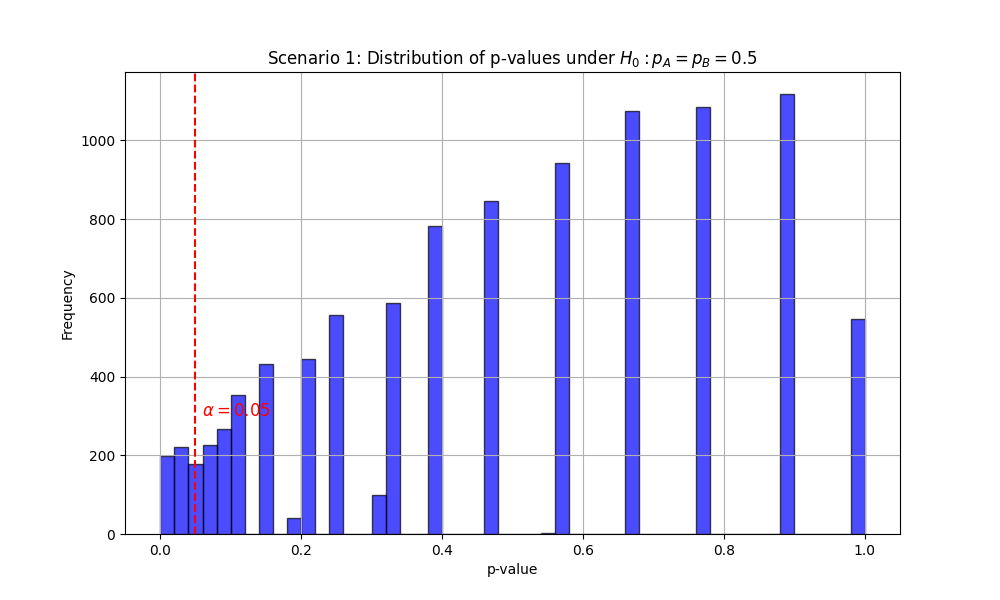
\includegraphics[width=0.8\textwidth]{scenario1_pvalues.png}
	\caption{Scenario 1: Distribution of p-values under \( H_0: p_A = p_B = 0.5 \). The Type I error rate should approximate the significance level \( \alpha \).}
	\label{fig:scenario1}
\end{figure}

The observed Type I error rate closely matches the significance level \( \alpha = 0.05 \), indicating that the sequential test maintains its validity in this scenario.

\subsection{Scenario 2: Small Effect Size}

This scenario investigates the power of the sequential A/B test when there is a small but non-zero difference between the success probabilities (\( p_A = 0.5 \), \( p_B = 0.55 \)). We are particularly interested in how often the test correctly rejects the null hypothesis \( H_0: p_A = p_B \) in favor of the alternative \( H_1: p_A \neq p_B \).

\subsubsection{Simulation Results}

Figure~\ref{fig:scenario2} illustrates the power curve as a function of the sample size, showing the relationship between the sample size and the probability of correctly rejecting the null hypothesis.

\begin{figure}[H]
	\centering
%	\includegraphics[width=0.8\textwidth]{scenario2_power.png}
	\caption{Scenario 2: Power curve for detecting a small effect size (\( \Delta = 0.05 \)). The power increases with the sample size, demonstrating the sensitivity of the test.}
	\label{fig:scenario2}
\end{figure}

The results indicate that the power of the test increases with the sample size, as expected, but the sequential approach allows for earlier detection of differences compared to a fixed-sample test.

\subsection{Scenario 3: Sequential Analysis with Stopping Rules}

In this scenario, we simulate a more dynamic environment where the data is analyzed sequentially, and the test can stop early if strong evidence is found for either \( H_0 \) or \( H_1 \). We use stopping boundaries defined by thresholds on the log-likelihood ratio.

\subsubsection{Simulation Results}

Figure~\ref{fig:scenario3} shows the distribution of stopping times (i.e., the number of samples required to reach a decision) and the resulting error rates.

\begin{figure}[H]
	\centering
%	\includegraphics[width=0.8\textwidth]{scenario3_stopping_times.png}
	\caption{Scenario 3: Distribution of stopping times in a sequential A/B test. The test often stops early, reducing the average sample size needed to reach a decision.}
	\label{fig:scenario3}
\end{figure}

The simulation results demonstrate that the sequential test can significantly reduce the required sample size while maintaining appropriate error rates. This highlights the efficiency of the sequential approach, especially in real-time A/B testing environments.

\subsection{Scenario 4: Average Stopping Time in Sequential A/B Testing}

In this scenario, we focus on the average stopping time of a sequential A/B test, which is a critical factor in evaluating the efficiency of sequential testing methods. The stopping time refers to the number of observations required for the test to reach a decision—either to accept or reject the null hypothesis—based on the accumulated evidence.

\subsubsection{Simulation Setup}

The stopping time is influenced by several factors, including the effect size \( \Delta = p_B - p_A \), the sample sizes \( n_A \) and \( n_B \), and the thresholds used for early stopping. In this simulation, we vary the effect size and sample sizes while maintaining a fixed significance level \( \alpha = 0.05 \).

\begin{itemize}
	\item \textbf{Effect Sizes}: We consider a range of effect sizes, including small (\( \delta = 0.01 \)), moderate (\( \delta = 0.05 \)), and large (\( \delta = 0.1 \)).
	\item \textbf{Sample Sizes}: The initial sample sizes \( n_A = n_B = 50 \) are used, with increments of 10 as the test progresses.
	\item \textbf{Stopping Criteria}: The test stops early if the log-likelihood ratio exceeds predefined thresholds corresponding to a significance level of \( \alpha = 0.05\) and power \( 1 - \beta = 1 - 0.05  \).
\end{itemize}
%TODO zmienic alpha /beta na I i II error

\subsubsection{Simulation Procedure}

The simulation is conducted by generating Bernoulli-distributed outcomes for both groups A and B with success probabilities \( p_A \) and \( p_B \). The sequential A/B test is applied, and the stopping time \( T \) is recorded for each simulation run. This process is repeated 10,000 times for each set of parameters to obtain a reliable estimate of the average stopping time.

The log-likelihood ratio at each stage \( t \) is calculated as:

\[
\log \left(\frac{p_1^t}{p_0^t}\right) = t(\bar{Y}_t - \bar{X}_t)\delta,
\]

where \( \bar{X}_t \) and \( \bar{Y}_t \) are the empirical averages of successes in groups A and B at time \( t \), respectively.

\subsubsection{Simulation Results}

The average stopping time \( \mathbb{E}[T] \) is computed for each combination of effect size and sample size. Figure~\ref{fig:avg_stopping_time} presents the results, showing how the average stopping time decreases as the effect size increases.

\begin{figure}[H]
	\centering
%	\includegraphics[width=0.8\textwidth]{avg_stopping_time.png}
	\caption{Average stopping time \( \mathbb{E}[T] \) as a function of effect size \( \Delta \) for different sample sizes. The results show that larger effect sizes lead to quicker decisions, reducing the average number of observations needed.}
	\label{fig:avg_stopping_time}
\end{figure}

As expected, the results indicate that the average stopping time decreases as the effect size increases. For larger effect sizes (\( \Delta = 0.1 \)), the test often concludes early, while smaller effect sizes (\( \Delta = 0.01 \)) require more observations before reaching a decision. This highlights the efficiency of sequential testing in identifying significant differences quickly, especially when the true effect size is large.

\begin{table}
	\caption{Summary of Selected Data}
	\label{tab:selected_data_summary}
	\begin{tabular}{l*{9}{c}}
		\hline \hline
		\textbf{$\tau$} & 0.1 & 0.2& 0.3& 0.4 & 0.45 & 0.47 & 0.48 & 0.49 \\
		\hline
		\textbf{mean} & 37.69 & 50.21 & 75.92 & 149.46 & 269.08 & 355.41 & 398.96 & 426.36 \\
		\textbf{std} & 8.92 & 15.40 & 29.84 & 81.40 & 192.76 & 266.59 & 321.06 & 336.41 \\
		\textbf{min} & 18.00 & 19.00 & 22.00 & 31.00 & 34.00 & 33.00 & 23.00 & 37.00 \\
		\textbf{25\%} & 31.00 & 40.00 & 55.00 & 91.00 & 136.00 & 167.00 & 179.00 & 186.00 \\
		\textbf{50\%} & 37.00 & 48.00 & 70.00 & 130.00 & 217.00 & 280.00 & 298.00 & 330.00 \\
		\textbf{75\%} & 43.00 & 58.00 & 91.00 & 188.00 & 349.25 & 459.00 & 529.00 & 567.25 \\
		\textbf{max} & 86.00 & 122.00 & 232.00 & 613.00 & 1672.00 & 2143.00 & 2521.00 & 2445.00 \\
		\textbf{Error Rate} & 0.00 & 0.00 & 0.00 & 0.00 & 0.06 & 0.14 & 0.22 & 0.37 \\
		\hline \hline
	\end{tabular}
\end{table}

\bibliographystyle{bibliografia_styl}
\bibliography{bibliografia}
\end{document}